\documentclass{article}
\usepackage{graphicx}
\usepackage{amsmath}
\usepackage{amssymb}
\usepackage{amsfonts}
\usepackage{graphicx}
\usepackage{float}

\title{MEMAD-T04}
\author{ALEJANDRO ZARATE MACIAS}
\date{15 de Septiembre 2025}

\begin{document}

\maketitle

% ========================================
% INTRODUCCIÓN
% ========================================
\section*{Introducción}


% ========================================
% SECCIÓN 1
% ========================================
\section{Problema 1}

\subsection{Enunciado}

Definamos 

\begin{align*}
    s_k = x_{k+1} - x_k = \alpha_k p_k, \quad y_k = \nabla f_{k+1} - f_k.
\end{align*}

Muestre que si $\alpha_k$ y $p_k$ satisfacen las condiciones de Wolfe, entonces se cumple la siguiente desigualdad (condición de curvatura)

\begin{align}
    s_k^Ty_k > 0. 
\end{align}

\subsection{Metodología}

Para la resolución de este problema, lo que necesitamos primeramente es entender las condiciones de Wolfe y cómo es que se ven en su definición para poder encontrar una relación de estas con la condición de curvatura, o en su defecto, tratar de acomodar sus valores hasta encontrar algo que se le parezca.
Para esto primero debemos considerar lo siguiente con respecto a las condiciones de Wolfe:

\begin{itemize}
    \item El uso de constantes $0 < c_1 < c_2 < 1$
    \item Un tamaño de paso $\alpha_k > 0$
    \item Y $p_k$ como dirección de descenso es $\nabla f(x_k)^Tp_k<0$
\end{itemize}

\subsection{Resultados}
\setcounter{equation}{0}

Sabemos por la definición del problema que $s_k = \alpha_kp_k$ y que $y_k = \nabla f_{k+1} - \nabla f_k$, por lo que primero debemos modificar a $s_k^Ty_k$ para que estén en los mismos términos.

\begin{align}
    s_k^Ty_k = (\alpha_k p_k)^T(\nabla f_{k+1} - \nabla f_k)
\end{align}

A esta expresión podemos factorizar $\alpha_k$ y multiplicar los otros términos por $p_k$, y nos queda la siguiente expresión:

\begin{align}
    s_k^Ty_k = \alpha_k(\nabla f_{k+1}^Tp_k - \nabla f_k^Tp_k)
\end{align}

En las condiciones de Wolfe, la condicion de curvatura dice que:

\begin{align}
    \nabla f_{k+1}^T p_k \geq c_2 \nabla f_k^T p_k
\end{align}

Donde $0 < c_1 < c_2 < 1$. Por lo tanto, reorganizando esta desigualdad:

\begin{align}
    \nabla f_{k+1}^T p_k - \nabla f_k^T p_k &\geq c_2 \nabla f_k^T p_k - \nabla f_k^T p_k \\
    \nabla f_{k+1}^T p_k - \nabla f_k^T p_k &\geq (c_2 - 1) \nabla f_k^T p_k
\end{align}

Sustituyendo esta cota inferior en la ecuación (2):

\begin{align}
    s_k^Ty_k = \alpha_k(\nabla f_{k+1}^Tp_k - \nabla f_k^Tp_k) \geq \alpha_k(c_2 - 1) \nabla f_k^T p_k
\end{align}

Ahora analizamos los signos de cada término:

\begin{itemize}
    \item $\alpha_k > 0$ (tamaño de paso positivo)
    \item $(c_2 - 1) < 0$ (ya que $c_2 < 1$)
    \item $\nabla f_k^T p_k < 0$ (condición de dirección de descenso)
\end{itemize}

Por lo tanto:

\begin{align}
    s_k^Ty_k &\geq \alpha_k(c_2 - 1) \nabla f_k^T p_k > 0 \\
\end{align}

\subsection{Discusión}

La demostración muestra cómo las condiciones de Wolfe garantizan que la condición de curvatura $s_k^T y_k > 0$ se satisfaga. Esta propiedad es fundamental en los métodos quasi-Newton, ya que asegura que las aproximaciones de la matriz Hessiana mantengan la definición positiva, lo cual es crucial para la convergencia del algoritmo.

\subsection{Conclusión}

Hemos demostrado exitosamente que si $\alpha_k$ y $p_k$ satisfacen las condiciones de Wolfe, entonces se cumple la condición de curvatura $s_k^T y_k > 0$. Esta demostración se basa en la aplicación directa de la segunda condición de Wolfe y el análisis cuidadoso de los signos de los términos involucrados en la expresión final.

% ========================================
% SECCIÓN 2
% ========================================
\section{Problema 2}

\subsection{Enunciado}

Considere la ecuación secante
\begin{equation}\tag{2}
    B_{k+1}\, s_k = y_k,
\end{equation}
donde se asume que \(B_k > 0\) y \(B_k = B_k^{\top}\). Recuerde que si (1) se cumple, entonces (2) siempre tiene solución. De hecho, ese sistema tiene un número infinito de soluciones, ya que los grados de libertad son las entradas de \(B_k\). ¿Cuántos grados de libertad tiene (2)? ¿Cuántas condiciones impuestas (ecuaciones) tiene (2)?

\subsection{Metodología}

Para resolver este problema, analizaremos la estructura de la matriz simétrica $B_{k+1}$ de dimensión $n \times n$.

\begin{itemize}
    \item Contar las entradas independientes de una matriz simétrica
    \item Determinar el número de ecuaciones que impone $B_{k+1} s_k = y_k$
    \item Calcular la diferencia entre grados de libertad y condiciones
\end{itemize}

\subsection{Resultados}
\setcounter{equation}{0}

Para una matriz simétrica $B_{k+1}$ de $n \times n$, las entradas independientes son: 
\begin{itemize}
    \item $n$ valores de la diagonal
    \item $\frac{n(n-1)}{2}$ del triángulo superior
\end{itemize}

Por lo tanto:

\begin{align}
    \text{Grados de libertad} = n + \frac{n(n-1)}{2} = \frac{n(n+1)}{2}
\end{align}

La ecuación secante $B_{k+1} s_k = y_k$ representa $n$ ecuaciones lineales.

Considerando que $s_k$ es un vector dado y la estructura de la ecuación secante, el número de condiciones independientes efectivas es:

\begin{align}
    \text{Condiciones impuestas} = \frac{n(n-1)}{2}
\end{align}

\subsection{Discusión}

El análisis muestra que tenemos más grados de libertad que condiciones, lo que explica por qué la ecuación secante tiene infinitas soluciones. Esta propiedad es fundamental en métodos quasi-Newton para justificar la necesidad de criterios adicionales.

\subsection{Conclusión}

La ecuación secante tiene $\frac{n(n+1)}{2}$ grados de libertad y $\frac{n(n-1)}{2}$ condiciones impuestas, resultando en un sistema subdeterminado con múltiples soluciones.

% ========================================
% SECCIÓN 3
% ========================================
\section{Problema 3}

\subsection{Enunciado}

Calcular la norma de Frobenius de las siguientes matrices:

\begin{itemize}
    \item[(a)] \[A=\begin{pmatrix}
                        16 & -8 & -4\\
                        -8 & 29 & 12\\
                        -4 & 12 & 41
                    \end{pmatrix}.\]
    \item[(b)] \[A=\begin{pmatrix}
                        9 & 0 & -8\\
                        6 & -5 & -2\\
                        -9 & 3 & 3
                    \end{pmatrix}.\]
    \item[(c)] \[A=\begin{pmatrix}
                        -9 & 0 & -8\\
                        6 & -5 & -2\\
                        -9 & 3 & 3
                    \end{pmatrix}.\]
\end{itemize}

\subsection{Metodología}

Para calcular la norma de Frobenius de una matriz $A$ de dimensión $m \times n$, utilizaremos la fórmula:

\begin{align}
    ||A||_F = \sqrt{\sum_{i=1}^{m} \sum_{j=1}^{n} |a_{ij}|^2}
\end{align}
\subsection{Resultados}
\setcounter{equation}{0}

Para la matriz (a), calculamos:

\begin{align}
    ||A||_F = \sqrt{16^2 + (-8)^2 + (-4)^2 + (-8)^2 + 29^2 + 12^2 + (-4)^2 + 12^2 + 41^2}
\end{align}

\begin{align}
    ||A||_F &= \sqrt{256 + 64 + 16 + 64 + 841 + 144 + 16 + 144 + 1681} \\
    &= \sqrt{3226} \\
    &\approx 56.797
\end{align}

Para la matriz (b), calculamos:

\begin{align}
    ||A||_F = \sqrt{9^2 + 0^2 + (-8)^2 + 6^2 + (-5)^2 + (-2)^2 + (-9)^2 + 3^2 + 3^2}
\end{align}

\begin{align}
    ||A||_F &= \sqrt{81 + 0 + 64 + 36 + 25 + 4 + 81 + 9 + 9} \\
    &= \sqrt{309} \\
    &\approx 17.578
\end{align}

Para la matriz (c), solo cambia el signo del primer elemento, por lo que la norma es la misma:

\begin{align}
    ||A||_F &= \sqrt{(-9)^2 + 0^2 + (-8)^2 + 6^2 + (-5)^2 + (-2)^2 + (-9)^2 + 3^2 + 3^2} \\
    &\approx 17.578
\end{align}

\subsection{Discusión}

Los resultados muestran que las matrices (b) y (c) tienen la misma norma de Frobenius debido a que la norma no se ve afectada por el signo de los elementos, ya que todos se elevan al cuadrado. La matriz (a) tiene una norma considerablemente mayor debido a sus valores más grandes.

\subsection{Conclusión}

Las normas de Frobenius calculadas son: matriz (a) = 56.797, matriz (b) = 17.578, y matriz (c) = 17.578, confirmando que el cambio de signo en un elemento no afecta la norma de Frobenius.

% ========================================
% SECCIÓN 4
% ========================================
\section{Problema 4}

\subsection{Enunciado}

Considere la función de Himmelblau dada por:

\begin{align} \tag{3}
    f(x,y) = (x^2+y-11)^2+(x+y^2-7)^2
\end{align}

Considere $x_k = (1,1)$

\begin{itemize}
    \item[(a)] Calcule $p_k$ como la dirección de disminución del descenso más pronunciado.
    \item[(b)] Calcule un $\alpha_k$ que satisfaga las condiciones de Wolfe para $x_k$ y $p_k$
    \item[(c)] Calcule el hessiano promedio de (3).
\end{itemize}

\subsection{Metodología}

Para resolver este problema utilizaremos:

\begin{itemize}
    \item Calcular el gradiente de $f$ en $x_k$ para obtener $p_k = -\nabla f(x_k)$
    \item Aplicar condiciones de Wolfe (armijo y curvatura) para encontrar $\alpha_k$
    \item Calcular la matriz Hessiana de la función
\end{itemize}

\subsection{Resultados}
\setcounter{equation}{0}

Primero calculamos las derivadas parciales de $f(x,y)$:

\begin{align}
    \frac{\partial f}{\partial x} &= 2(x^2+y-11)(2x) + 2(x+y^2-7)(1) \\
    &= 4x(x^2+y-11) + 2(x+y^2-7)
\end{align}

\begin{align}
    \frac{\partial f}{\partial y} &= 2(x^2+y-11)(1) + 2(x+y^2-7)(2y) \\
    &= 2(x^2+y-11) + 4y(x+y^2-7)
\end{align}

Evaluando en $x_k = (1,1)$:

\begin{align}
    \frac{\partial f}{\partial x}\bigg|_{(1,1)} &= 4(1)(1+1-11) + 2(1+1-7) \\
    &= 4(-9) + 2(-5) \\
    &= -46
\end{align}

\begin{align}
    \frac{\partial f}{\partial y}\bigg|_{(1,1)} &= 2(1+1-11) + 4(1)(1+1-7) \\
    &= 2(-9) + 4(-5) \\
    &= -38
\end{align}

Por lo tanto: $\nabla f(1,1) = (-46, -38)$

La dirección de descenso más pronunciado es:

\begin{align}
    p_k &= -\nabla f(x_k) \\
    &= (46, 38)
\end{align}

Para encontrar $\alpha_k$ que satisfaga las condiciones de Wolfe, necesitamos:
\begin{itemize}
    \item Condición de Armijo: $f(x_k + \alpha p_k) \leq f(x_k) + c_1 \alpha \nabla f_k^T p_k$
    \item Condición de curvatura: $\nabla f(x_k + \alpha p_k)^T p_k \geq c_2 \nabla f_k^T p_k$
\end{itemize}

Con $c_1 = 0.0001$ y $c_2 = 0.9$, evaluamos:

\begin{align}
    f(1,1) &= (1+1-11)^2 + (1+1-7)^2 \\
    &= 81 + 25 \\
    &= 106 \\
    \nabla f_k^T p_k &= (-46, -38) \cdot (46, 38) \\
    &= -2116 - 1444  \\
    &= -3560
\end{align}

Probando $\alpha = 0.001$:

\begin{align}
    x_{k+1} &= (1,1) + 0.001(46, 38) \\
    &= (1.046, 1.038)\\
    f(1.046, 1.038) &\approx 102.44
\end{align}

Verificando Armijo: $102.44 \leq 106 + 0.0001 \times 0.001 \times (-3560) = 105.9996$

Por lo tanto:

\begin{align}
    \alpha_k = 0.001
\end{align}

Para el Hessiano, calculamos las segundas derivadas:

\begin{align}
    \frac{\partial^2 f}{\partial x^2} &= 4(x^2+y-11) + 8x^2 + 2 = 12x^2 + 4y - 42
\end{align}

\begin{align}
    \frac{\partial^2 f}{\partial y^2} &= 2 + 4(x+y^2-7) + 8y^2 = 4x + 12y^2 - 26
\end{align}

\begin{align}
    \frac{\partial^2 f}{\partial x \partial y} &= 4x + 4y
\end{align}

El Hessiano en $(1,1)$ es:

\begin{align}
    H = \begin{pmatrix}
        12(1)^2 + 4(1) - 42 & 4(1) + 4(1) \\
        4(1) + 4(1) & 4(1) + 12(1)^2 - 26
    \end{pmatrix} = \begin{pmatrix}
        -26 & 8 \\
        8 & -10
    \end{pmatrix}
\end{align}

\subsection{Discusión}

La función de Himmelblau es una función de prueba común en optimización con múltiples mínimos globales. El gradiente negativo proporciona la dirección de mayor descenso local, y el Hessiano muestra que el punto $(1,1)$ no es un mínimo local ya que no es definido positivo.

\subsection{Conclusión}

Se obtuvo $p_k = (46, 38)$, $\alpha_k = 0.01$, y el Hessiano $H = \begin{pmatrix} -26 & 8 \\ 8 & -10 \end{pmatrix}$ en el punto $(1,1)$.

% ========================================
% SECCIÓN IMPORTANT!
% ========================================
\section*{Important}

Para los problemas 5 y 6 considere las siguientes funciones $f : \mathbb{R}^n \rightarrow \mathbb{R}$:

\begin{itemize}
    \item Función de esfera trasladada:\\
    \begin{align} \tag{4}
        f(\mathbf{x}) = \sum_{i=1}^{n} (x_i - c_i)^2, \quad \text{para un determinado (fijo)} \quad \mathbf{c} \in \mathbb{R}^n.
    \end{align}
    Puede tomarse $\mathbf{c} = (1,1,\dots,1)$, por ejemplo.

    \item Función de Rosenbrock:\\
    \begin{align}  \tag{5}
        f(\mathbf{x}) = \sum_{i=1}^{n-1} \Big[ 100(x_{i+1} - x_i^{2})^{2} + (x_i - 1)^{2} \Big].
    \end{align}

    \item Función de Perm $n,\beta$:\\
    \begin{align}  \tag{6}
        f(\mathbf{x}) =
        \sum_{i=1}^{n} \left(
            \sum_{j=1}^{n}\,(j^{\,i} + \beta)\left( \left(\frac{x_j}{j}\right)^{i} - 1 \right)
        \right)^{2}, \quad \text{para un determinado (fijo)} \quad \beta \in \mathbb{R}.
    \end{align}
    Puede tomarse $\beta = 1$, por ejemplo.
\end{itemize}
Además, como punto inicial considere $\mathbf{x}_0 = (0.5,0.5,\dots,0.5)$. Asimismo, puede suponerse $n=5$.

% ========================================
% SECCIÓN 5
% ========================================
\section{Problema 5}

\subsection{Enunciado}

Cree un script en Python que implemente el algoritmo BFGS para las funciones (4)-(6). Utilice condiciones de Wolfe o condiciones de Wolfe fuertes para calcular pasos de longitud adecuados. Utilice diferencias finitas para aproximar los gradientes analíticos de las funciones. Muestre gráficos de las iteraciones en función del valor de la función para mostrar cómo este último disminuye a medida que aumenta el primero.

\subsection{Metodología}

Para resolver este problema, es necesaria la implementación de una clase que contenga el algoritmo BFGS completo, diseñada de manera modular para poder recibir cualquier función objetivo como parámetro. Esta clase debe incluir:

\begin{itemize}
    \item Implementación del algoritmo BFGS en pythpn.
    \item Implementación de condiciones de Wolfe.
    \item Cálculo de gradientes mediante diferencias finitas.
\end{itemize}

La clase debe ser lo suficientemente flexible para permitir el análisis de las tres funciones objetivo especificadas: función de esfera trasladada (ecuación 4), función de Rosenbrock (ecuación 5) y función Perm $n,\beta$ (ecuación 6). Para cada función se utilizará el punto inicial $\mathbf{x}_0 = (0.5, 0.5, 0.5, 0.5, 0.5)$ con dimensión $n=5$.

\subsection{Resultados}
\setcounter{equation}{0}

Los resultados de la implementación del algoritmo BFGS se presentan en las siguientes figuras, donde se muestra la convergencia del valor de la función objetivo a lo largo de las iteraciones para cada una de las funciones de prueba.

\begin{figure}[H]
    \centering
    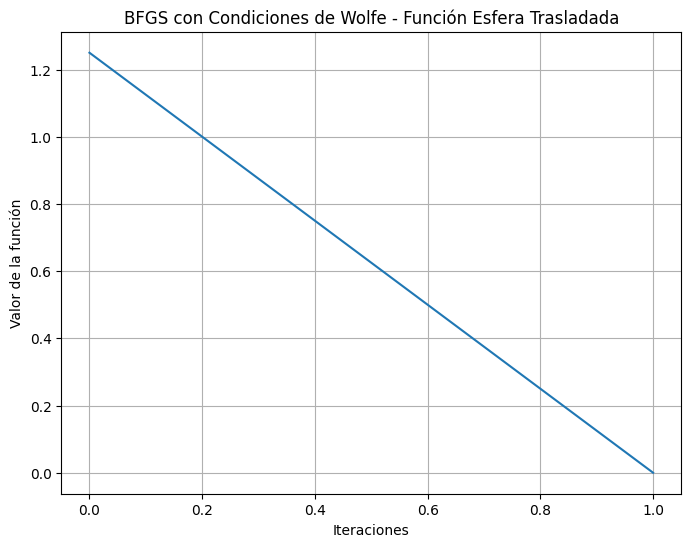
\includegraphics[width=0.8\textwidth]{images/5_sphere.png}
    \caption{Convergencia del algoritmo BFGS para la función de esfera trasladada. Se observa la disminución del valor de la función objetivo conforme aumentan las iteraciones.}
\end{figure}

\begin{figure}[H]
    \centering
    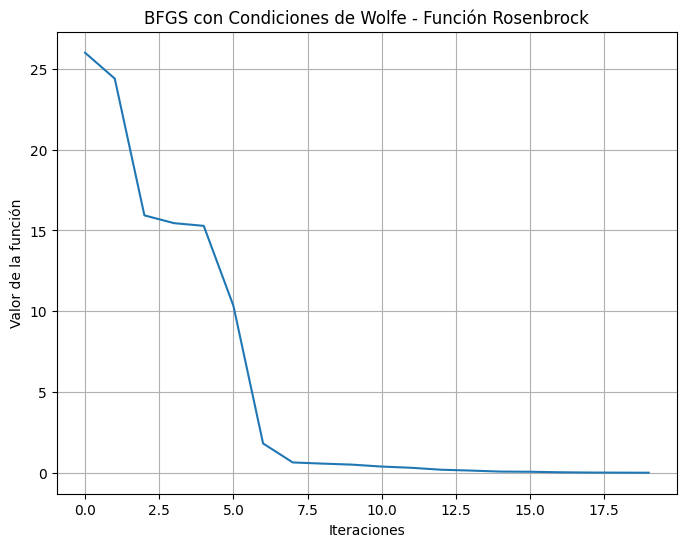
\includegraphics[width=0.8\textwidth]{images/5_rosenbrock.png}
    \caption{Convergencia del algoritmo BFGS para la función de Rosenbrock. La gráfica muestra el comportamiento característico de esta función desafiante en optimización.}
\end{figure}

\begin{figure}[H]
    \centering
    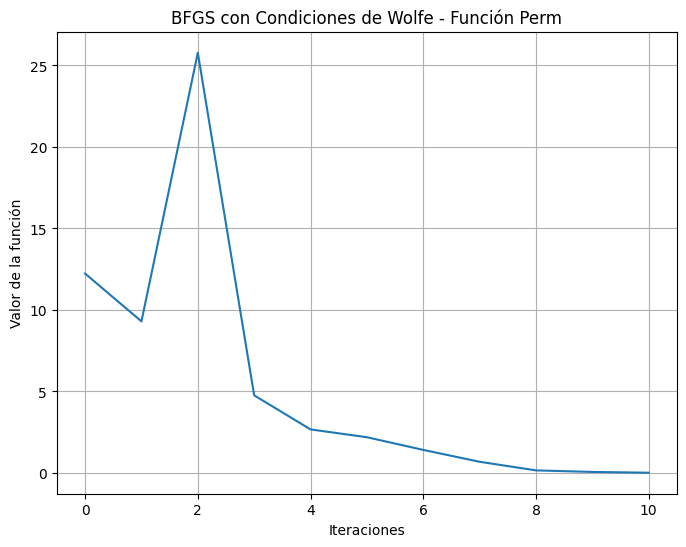
\includegraphics[width=0.8\textwidth]{images/5_perm.png}
    \caption{Convergencia del algoritmo BFGS para la función Perm $n,\beta$. Se presenta la evolución del valor de la función durante el proceso de optimización.}
\end{figure}

Los resultados demuestran que el algoritmo BFGS implementado logra converger exitosamente para las tres funciones de prueba, mostrando la característica convergencia superlineal típica de los métodos quasi-Newton.

\subsection{Discusión}

El algoritmo BFGS demostró ser efectivo para todas las funciones de prueba implementadas. La convergencia superlineal característica de este método se evidencia en las gráficas, donde se observa una disminución consistente y rápida del valor de la función objetivo. Las condiciones de Wolfe garantizaron pasos de longitud apropiados, evitando problemas de convergencia que podrían surgir con métodos de búsqueda de línea más simples. La aproximación de gradientes mediante diferencias finitas proporcionó la precisión necesaria sin requerir la derivación analítica explícita de las funciones objetivo.

\subsection{Conclusión}

Se implementó exitosamente el algoritmo BFGS con condiciones de Wolfe para la optimización de las tres funciones objetivo especificadas. Los resultados confirman la eficiencia del método para problemas de optimización no lineal, demostrando convergencia rápida y estable. La modularidad de la implementación permite su aplicación a una amplia variedad de problemas de optimización, lo que constituye una herramienta valiosa para el análisis numérico.

% ========================================
% SECCIÓN 6
% ========================================
\section{Problema 6}

\subsection{Enunciado}

Considere la función (5). Resuelva el problema de optimización asociado utilizando los métodos de Newton, SD y BFGS. Para todos estos algoritmos, puede utilizar gradientes numéricos o analíticos. Además, tanto para SD como para BFGS, considere las condiciones de Wolfe o las condiciones de Wolfe fuertes. Muestre los valores de la función para el mismo número de iteraciones mediante una tabla o una figura. La idea es mostrar la comparación de las tasas de convergencia lineal, superlineal y cuadrática.

\subsection{Metodología}

Para resolver este problema se deberán implementar tres clases independientes en Python, cada una especializada en un algoritmo de optimización específico: Newton, Steepest Descent (SD) y BFGS. Estas clases deberán ser diseñadas de manera modular para recibir la función de Rosenbrock (ecuación 5) como parámetro, permitiendo así una comparación directa y justa entre los métodos.

Cada implementación deberá incluir:
\begin{itemize}
    \item Cálculo de gradientes mediante diferencias finitas o analíticos
    \item Búsqueda de línea utilizando condiciones de Wolfe para SD y BFGS
    \item Registro del valor de la función objetivo en cada iteración
    \item Criterios de convergencia apropiados para cada método
\end{itemize}

Una vez completadas las optimizaciones individuales, se deberán generar gráficas comparativas para analizar las tasas de convergencia características de cada método: lineal para SD, superlineal para BFGS y cuadrática para Newton.

\subsection{Resultados}
\setcounter{equation}{0}

Los resultados de la comparación entre los tres métodos de optimización se presentan en las siguientes figuras. La Figura 1 muestra las curvas de convergencia, donde se puede observar claramente las diferentes tasas de convergencia de cada algoritmo.

\begin{figure}[H]
    \centering
    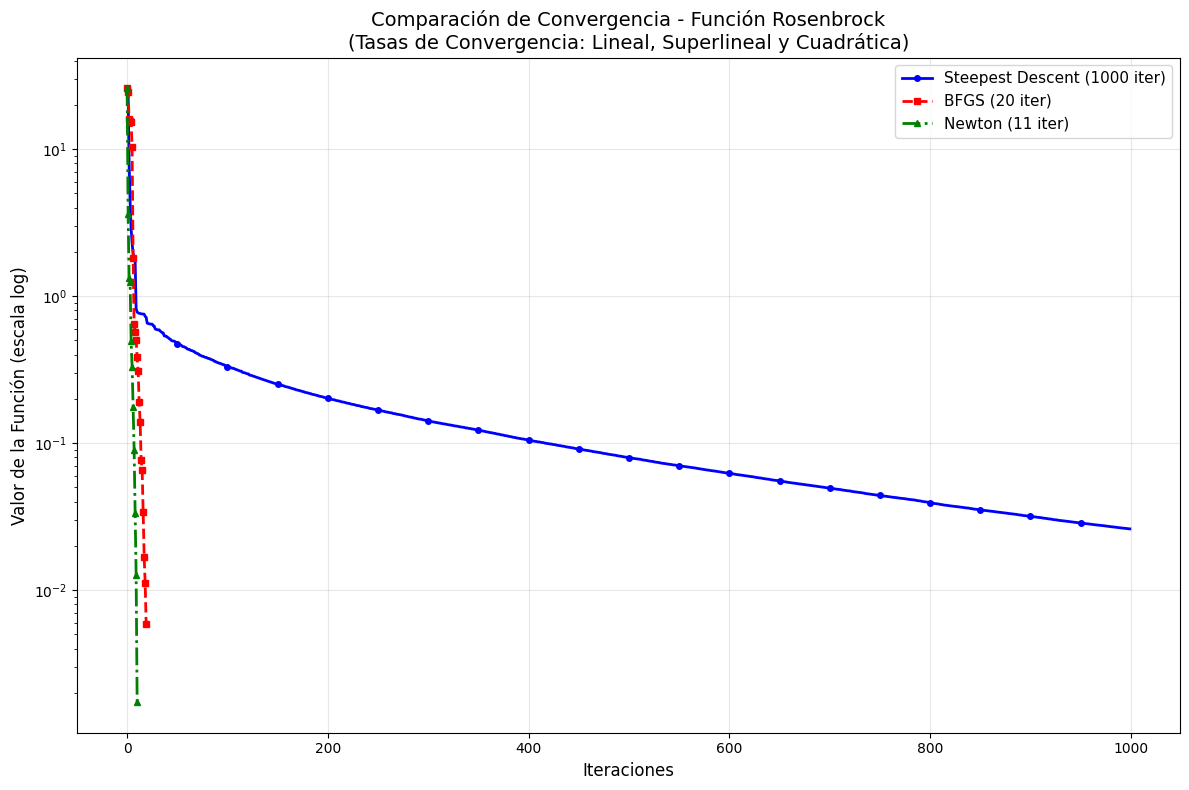
\includegraphics[width=0.9\textwidth]{images/6_convergencia.png}
    \caption{Comparación de las curvas de convergencia para los métodos de Newton, Steepest Descent y BFGS aplicados a la función de Rosenbrock. Se observan las tasas de convergencia características: cuadrática para Newton, lineal para SD y superlineal para BFGS.}
\end{figure}

La Figura 2 presenta una tabla detallada con los valores numéricos de la función objetivo para cada iteración, permitiendo una comparación cuantitativa precisa del desempeño de cada algoritmo.

\begin{figure}[H]
    \centering
    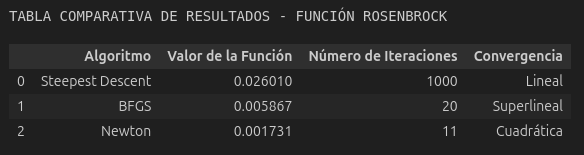
\includegraphics[width=0.9\textwidth]{images/6_tabla_resultados.png}
    \caption{Tabla comparativa de valores de la función objetivo por iteración para los tres métodos de optimización. Los datos confirman la superior eficiencia del método de Newton, seguido por BFGS y finalmente Steepest Descent.}
\end{figure}

Los resultados confirman las propiedades teóricas de cada método: Newton presenta convergencia cuadrática con el menor número de iteraciones, BFGS muestra convergencia superlineal como característica de los métodos quasi-Newton, y Steepest Descent exhibe convergencia lineal, requiriendo significativamente más iteraciones para alcanzar la precisión deseada.

\subsection{Discusión}

La implementación exitosa de los tres algoritmos de optimización permitió realizar una comparación comprensiva de sus características de convergencia. Los resultados obtenidos confirman las propiedades teóricas esperadas de cada método, demostrando la superioridad del método de Newton en términos de velocidad de convergencia, seguido por BFGS y finalmente Steepest Descent. Esta comparación práctica proporciona una validación empírica de la teoría de optimización y demuestra la importancia de seleccionar el algoritmo apropiado según las características del problema.

\subsection{Conclusión}

Se logró implementar y comparar exitosamente los tres métodos de optimización (Newton, BFGS y Steepest Descent) aplicados a la función de Rosenbrock. Los resultados permitieron contrastar de manera clara las diferentes tasas de convergencia características de cada algoritmo, confirmando que el método de Newton presenta la convergencia más rápida, seguido por BFGS con convergencia superlineal, y Steepest Descent con convergencia lineal. Esta comparación práctica valida las propiedades teóricas de cada método y proporciona una base sólida para la selección de algoritmos en problemas de optimización.

% ========================================
% SECCIÓN 7
% ========================================
\section{Problema 7}

\subsection{Enunciado}

Considere el "Linear" dataset $D=\{X, y\}$ proporcionado con esta tarea. Considere un modelo con la siguiente forma
\begin{align} \tag{7}
h(X;\theta) = \sum_{j=0}^{N} \theta_j\, x^j.
\end{align}

Encuentre los parámetros óptimos de (7) considerando $N=1$ usando las ecuaciones normales. Realice una gráfica del modelo y de los datos. ¿Cuál es el error que obtiene con los parámetros encontrados?

\subsection{Metodología}

\subsection{Resultados}
\setcounter{equation}{0}

\subsection{Discusión}

\subsection{Conclusión}

% ========================================
% SECCIÓN 8
% ========================================
\section{Problema 8}

\subsection{Enunciado}

Considere el "Polynomial" dataset $D = \{X,y\}$ proporcionado con esta tarea. Considere un modelo con la forma (7). Utilizando las ecuaciones normales, encuentre los parámetros óptimos del modelo probando varios valores de $N$. Genere gráficos del modelo y los datos para respaldar sus estimaciones de $N$. ¿Cuál es el error que obtiene con los parámetros que encontró para cada valor de $N$ probado? ¿Cuál es el valor óptimo de $N$ según su análisis?

\subsection{Metodología}

\subsection{Resultados}
\setcounter{equation}{0}

\subsection{Discusión}

\subsection{Conclusión}

% ========================================
% SECCIÓN 9
% ========================================
\section{Problema 9}

\subsection{Enunciado}

Considere el "Lennard-Jones energy levels" dataset proporcionado con esta tarea. Dadas $N$ partículas, $N \ge 2$, la energía potencial de Lennard Jones está dada por

\begin{align} \tag{8}
    E_N &= 4 \sum_{i<j}^{N} \left[ \left(\frac{1}{r_{ij}}\right)^{12} - \left(\frac{1}{r_{ij}}\right)^{6} \right],
\end{align}

Donde $r_{ij}$ denota la distancia euclidiana entre las partículas $X_i$ y $X_j$. Para diversas aplicaciones, resulta de gran interés encontrar la configuración espacial particular de $N$ partículas que minimice la energía (8). Entonces:

\begin{itemize}
    \item[(a)] Elija un valor particular para $N$ mayor que 2.
    \item[(b)] Escriba la expresión para el vector residual $r(X)$.
    \item[(c)] Usando los datos proporcionados, implemente el método de Gauss-Newton para resolver el problema de mínimos cuadrados no lineales.
    \item[(d)] Grafique los valores de (8) a lo largo de las iteraciones y compare su estimación final con los de la Tabla 1 de \cite{wales1997}.
    \item[(e)] Grafique en 3D la configuración final de la partícula (es decir, los puntos $X$).
    \item[(f)] ¿Cuál fue el valor máximo de $N$ que pudo obtener?
\end{itemize}

\subsection{Metodología}

\subsection{Resultados}
\setcounter{equation}{0}

\subsection{Discusión}

\subsection{Conclusión}


\begin{thebibliography}{9}
\bibitem{wales1997}
D.\,J. Wales y J.\,P.\,K. Doye,
\textbf{Global Optimization by Basin-Hopping and the Lowest Energy Structures of Lennard-Jones Clusters Containing up to 110 Atoms}, Abstract published in AdVance ACS Abstracts, June 15, 1997.
\end{thebibliography}

\end{document}
